As a basis for this project, the implementation of inverse planning on \url{https://github.com/stacyste/TheoryOfMindInferenceModels} was used.
The implementation was done in Python 3, and kept in the same language for this project. However, additions to the language from Python 3.9 are used.
To allow for expansion and the implementation of different methods, the code base was made modular.
Another method of representing states, and another way of navigating was implemented.
Furthermore, the implementation was sped up.
Moreover, a testing environment was created to ensure functionality of the original example scenarios and all expansions.
In the following, the main modules, its functionality, and usage will be explained.

\subsection{Dependencies}
The program has the following dependencies:
\begin{itemize}
	\setlength\itemsep{0em}
	\item numpy\footnote{numpy.org/}
	\item pandas\footnote{pandas.pydata.org/}
	\item matplotlib\footnote{matplotlib.org/}
	\item tqdm\footnote{tqdm.github.io/}
\end{itemize}

\subsection{Representation Types}
\subsubsection{Map-like Regular Grid Representation}
To represent the environment, the modeling approach in \citeA{baker2009} uses a regular grid map-like representation with 2D squares discretizing the environment.
This is a popular choice for navigation models (cf. e.g., \citeNP{algfoor2015}).

\subsubsection{Vector-based Representation}
The other representation type that was implemented in this project is a vector representation of the goals.
The states in the environment are discretized just like in the map-like representation. However, the agent has no access to the cell in the grid itself, and its position.
To the agent, the cell is a set of vectors that describe the distance and the direction to all goals in the environment.


\subsection{Loading Experimental Data}
A new module was created to allow the loading of experimental data into the program.
A full example of this can be found in the appendix in Section \ref{appendix:ex_loading}.

The module is developed to load data of the following form:
First, the configuration is specified using YAML \footnote{\url{yaml.org/}}.
In this configuration, the shape of the arena needs to be specified. Currently, two shapes are possible: circles and rectangles.

A circular arena is configured as follows.

\begin{verbatim}
	#     Circle:
	#       center_x: 4
	#       center_y: 4
	#       radius: 3
\end{verbatim}

The discrete cells which are included in the circular arena are calculated quadrant-wise. Around the center of the circle ($centerX, centerY$), all cells are included for which

\[
(x - centerX)^2 + (y - centerY)^2 < r
\]

\noindent
holds for the inner corner of the cell.

The center of the circle is transformed to $(0,0)$, so the discretization is independent of the center. This issue can be demonstrated with a simple example, as shown in Figure \ref{fig:circle_issue}. The resulting arena of the example configuration can be seen in Figure \ref{fig:circular_arena}.

\begin{figure}[htb]
	\centering
	\resizebox{0.95\linewidth}{!}{%
		\subcaptionbox{{\large Circle with center $(2,2)$ and radius $1.5$.}}{
			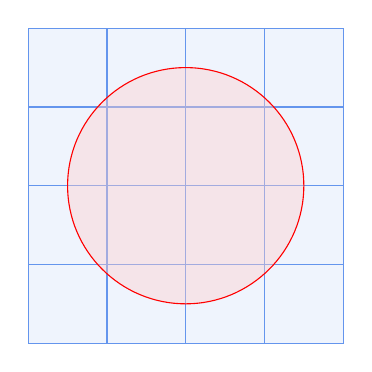
\begin{tikzpicture}
				\tkzInit[xmax=4,ymax=4,xmin=0,ymin=0]
				\begin{scope}[dotted]
					\tkzGrid[color=black!50, line width = 0.3pt]
				\end{scope}
				%\tkzGrid
				%\draw[ thick,latex-latex] (-1,4) -- (4,-6) node[anchor=south west] {$a$}; % two points for drawing 2x+y=2
				\foreach \x/\y in {1/1, 1/2, 1/3, 1/4, 2/1, 2/2, 2/3, 2/4, 3/1, 3/2, 3/3, 3/4, 4/1, 4/2, 4/3, 4/4}
				\filldraw[draw=CornflowerBlue,fill=CornflowerBlue!10, fill opacity=1] (\x-1,\y-1) rectangle (\x, \y);
				\filldraw[draw=red,fill=red!20, fill opacity=.4] (2,2) circle (1.5);
				\tkzAxeXY
			\end{tikzpicture}
		}%
		%\hfill
		\hspace{0.1\linewidth}
		\subcaptionbox{{\large Circle with center $(1.5,1.5)$ and radius $1.5$.}}{
			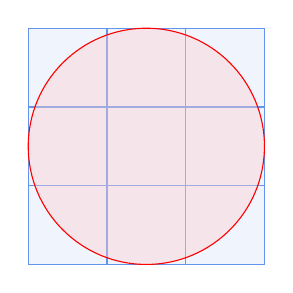
\begin{tikzpicture}
				\tkzInit[xmax=4,ymax=4,xmin=0,ymin=0]
				\begin{scope}[dotted]
					\tkzGrid[color=black!50, line width = 0.3pt]
				\end{scope}
				%\tkzGrid
				
				%\draw[ thick,latex-latex] (-1,4) -- (4,-6) node[anchor=south west] {$a$}; % two points for drawing 2x+y=2
				\foreach \x/\y in {1/1, 1/2, 1/3, 2/1, 2/2, 2/3, 3/1, 3/2, 3/3}
				\filldraw[draw=CornflowerBlue,fill=CornflowerBlue!10, fill opacity=1] (\x-1,\y-1) rectangle (\x, \y);
				\filldraw[draw=red,fill=red!20, fill opacity=.4] (1.5,1.5) circle (1.5);
				\tkzAxeXY
			\end{tikzpicture}
		}%
	}
	\caption{Discretization of circles can differ depending on the center.}
	\label{fig:circle_issue}
\end{figure}

\begin{figure}[htb]
	\begin{center}
		\resizebox{0.75\linewidth}{!}{%
			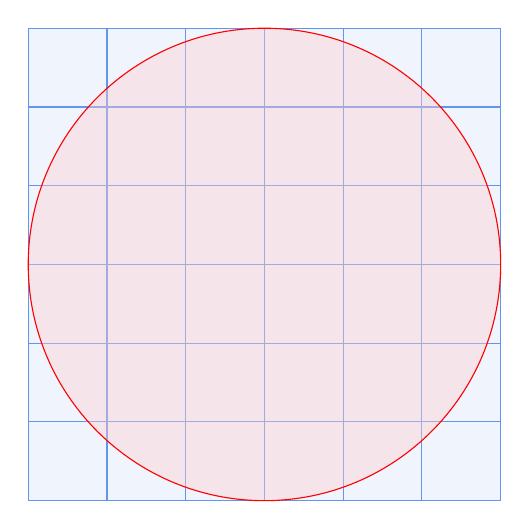
\begin{tikzpicture}
				\tkzInit[xmax=7,ymax=7,xmin=0,ymin=0]
				\begin{scope}[dotted]
					\tkzGrid[color=black!50, line width = 0.3pt]
				\end{scope}
				%\tkzGrid
				
				%\draw[ thick,latex-latex] (-1,4) -- (4,-6) node[anchor=south west] {$a$}; % two points for drawing 2x+y=2
				\foreach \x/\y in {1/3, 2/3, 1/6, 3/2, 2/6, 4/3, 3/5, 5/3, 4/6,
					6/2, 5/6, 6/5, 1/1, 2/1, 1/4, 3/6, 2/4, 4/1,
					3/3, 6/3, 5/1, 4/4, 6/6, 5/4, 4/2, 3/1, 1/2,
					3/4, 2/2, 1/5, 4/5, 6/1, 2/5, 5/5, 6/4, 5/2}
				\filldraw[draw=CornflowerBlue,fill=CornflowerBlue!10, fill opacity=1] (\x-1,\y-1) rectangle (\x, \y);
				\filldraw[draw=red,fill=red!20, fill opacity=.4] (3,3) circle (3);
				\tkzAxeXY
			\end{tikzpicture}
		}
	\end{center}
	\caption{Circular arena with a center at $(3, 3)$ and a radius of $3$. The center was transformed from the original $(4,4)$. The circle is approximated by including all discrete cells with at least one corner within the specified circle.}
	\label{fig:circular_arena}
\end{figure}

A rectangular arena is specified similarly:

\begin{verbatim}
	#     Rectangle:
	#       center_x: 4
	#       center_y: 4
	#       grid_width: 6
	#       grid_height: 6
\end{verbatim}

The center is transformed to $(grid\_width/2,grid_height/2)$, such that the lower left corner adheres to $(0,0)$. This gives an arena as expected, which is depicted in Figure \ref{fig:rect_arena}.

For both shapes, all specifications have to be $\geq$ 0.

\begin{figure}[htb]
	\centering
	\resizebox{0.75\linewidth}{!}{%
	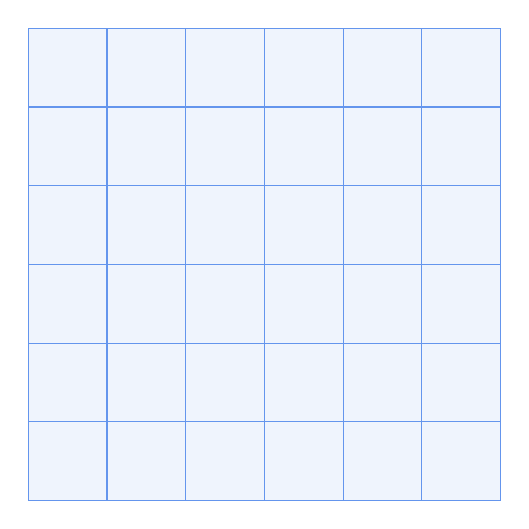
\begin{tikzpicture}
		\tkzInit[xmax=7,ymax=7,xmin=0,ymin=0]
		\begin{scope}[dotted]
			\tkzGrid[color=black!50, line width = 0.3pt]
		\end{scope}
		
		\foreach \x in {1,...,6}
			\foreach \y in {1,...,6}
				\filldraw[draw=CornflowerBlue,fill=CornflowerBlue!10] (\x-1,\y-1) rectangle (\x,\y);
		\tkzAxeXY
	\end{tikzpicture}
	}
	\caption{Rectangular arena created with the specifications of a center at $(0,0)$, transformed from $(4,4)$, a height of $6$ and a width of $6$.}
	\label{fig:rect_arena}
\end{figure}



After the YAML specification, the data file must contain position data from a single agent in a single trial.
This data is discretized to match the grid specified before.

The module \module{io} implements a reader class \module{CSVReader}, illustrated in Figure \ref{fig:uml:csvreader}, which provides the means to load this type of data.
The arena dimensions specified in the data file can be accessed via the \module{dimensions} function provided by the \module{CSVReader}. Currently this module can load arenas of circular and rectangular shapes.
The positional recordings can be accessed using the \module{trajectory} function.

\definecolor{classcolor}{HTML}{F3B3A9}
\tikzumlset{fill class=classcolor!30}
\begin{figure}
	\centering
\begin{tikzpicture}
		\umlclass[ ] {io::CSVReader}{
			data\_path : str \\ pixelation : int
		}{read() : pandas.DataFrame \\ raw\_data() : pandas.DataFrame \\ read\_partial(requirements) : pandas.DataFrame \\ dimensions() : dict \\ trajectory(pandas.DataFrame) : list}
\end{tikzpicture}
\caption{Class \module{CSVReader} is used to load trajectory data into the program, and parse settings from the file, such as the dimensions of the arena.}
\label{fig:uml:csvreader}
\end{figure}

Sometimes, e.g. due to performance requirements, it might be desired to increase the rasterization of the environment to reduce the overall number of cells in the grid.
This can be done using the optional initiation parameter \module{pixelation} for the \module{CSVReader} class (see Figure \ref{fig:uml:csvreader}).
By default, this parameter is set to $1$, meaning no downsampling of states is undertaken.
Higher values will result in a smaller problem space.

From the parsed environment dimensions, an \module{Environment} object can be created (see Figure \ref{fig:uml:environment}).
In this step, goals and obstacle positions need to be provided, with their positions adjusted to the in the loading step specified pixelation.
An example environment can be seen in Figure \ref{subfig:env}.
Goals should be specified as a \module{Goal} object, see Figure \ref{fig:uml:goal}.
These specifications are then combined to an \module{MDP} object (see Figure \ref{fig:uml:mdp}), which provides the methods to describe the problem as a Markov Decision Problem.

\begin{figure}
	\centering
		\begin{tikzpicture}
		\umlclass[ ] {model::Goal}{
			name : str \\ pos : tuple[int, int] \\ reward : float
		}{}
	\end{tikzpicture}
	\caption{Class \module{Goal} is used to represent a goal in the environment, with respective position and reward, as well as a name for readability.}
	\label{fig:uml:goal}
	\begin{tikzpicture}
		\umlclass[] {model::Environment}{
			goals : [Goal] \\ obstacles : [tuple[int, int]] \\
			coords : [tuple[int, int]]
		}{}
	\end{tikzpicture}
	\caption{Class \module{Environment} represents an experimental environment, including goals and obstacles.}
	\label{fig:uml:environment}
	
	\begin{tikzpicture}
	\umlclass[] {model::MDP}{
		environment : Environment \\
		T : all possible transitions in environment
	}{reward\_table() : mapping from T to rewards}
	\end{tikzpicture}
	\caption{Class \module{MDP} represents the theoretical foundations for solving an MDP.}
	\label{fig:uml:mdp}
\end{figure}

To make these steps easier, a specific type of model is provided which executes these steps autonomously.
The \module{DataModel} class, provided by the \module{Model} module, implements the loading and adjusting procedures.

\subsection{Data Sampling}

The second possibility is to sample a trajectory instead of loading it from data.
This is done via the \module{SamplingModel} class.
An example can be found in the appendix, Section  \ref{appendix:ex_sampling}.
The arena dimensions can be either loaded from a file with specified configurations, or defined manually.
No transformation is taking place, so the center needs to be defined as $(width/2, height/2)$, or $(radius, radius)$ for a circular arena.
Goals and obstacles have to be specified as described in the previous section on how to load experimental data.

Another required parameter is the starting position, which can be any position in the specified environment, and which can also be specified in a configuration file.

The class implements a method to sample a goal according to either specified goal priors, or a uniform distribution.
With a chosen goal, which can also be chosen manually be the modeler, the class can then sample trajectories using the method \module{sample\_trajectory}.
This is done using a policy over the environment.
This policy has to be calculated, which will be explained in the following.

\iffalse
\begin{figure}
	\begin{tikzpicture}
		\umlclass[ ] {model::SamplingModel}{
			dimensions : dict \\ goals : list \\ obstacles : list \\ start\_pos : 
		}{\_\_init\_\_(dimensions : dict, goals : list, obstacles : list, start\_pos : tuple[int, int])}
	\end{tikzpicture}
	\caption{\TODO{description} \TODO{simplified}, e.g. no agent class}
	\label{fig:uml:samplingmodel}
\end{figure}
\fi

\subsection{Policy Calculation}
Before policies can be calculated, the previously specified models are used to generate \module{MDP} objects, which provide methods that grant easy access to constructs used by MDP solving algorithms, such as the reward function, or the transition model.

Policies are calculated internally in the \module{Model} class and all its children using implementations of the \module{Solver} class, provided by the \module{calcs.mdp} package. 
The \module{Solver} class provides the function \module{calculate\_policies(goal : Goal, beta : float)}, which has to be implemented by inheriting classes, and calculates policies to a given goal, using the determinism factor beta ($\beta$ in Equation \ref{eq:boltzmann}).
Currently, two implementations exist: the \module{OptimalSolver} class (see Figure \ref{fig:uml:optimalsolver}), which implements the value iteration algorithm employed by \citeA{baker2009}, and the \module{GreedySolver}.
Utility values of the in an exemplary environment can be seen in Figure \ref{fig:utilities}. 

\paragraph{Optimal Solver.}

\begin{figure}
	\centering
	\begin{tikzpicture}
		\umlclass[ ] {calcs.mdp::OptimalSolver}{
			mdp : MDP \\ beta : float \\ utilities : dict \\ gamma : float \\ reward\_table : dict
		}{+\_\_init\_\_(mdp : MDP, gamma : float =.95) \\ +policies(goal : Goal) \\ -\_q\_value(state : State, action : tuple[int, int], goal : Goal) : float \\ -\_value\_iteration(goal : Goal) : dict \\ -\_get\_boltzmann\_policy(state: State, goal : Goal) : dict}
	\end{tikzpicture}
	\caption{The class \module{OptimalSolver} takes a description of a Markov Decision Problem (in the form of an \module{MDP} object), and solves it via value iteration.}
	\label{fig:uml:optimalsolver}
\end{figure}

A class diagram of the \module{OptimalSolver} can be seen in Figure \ref{fig:uml:optimalsolver}.
This module implements the method used in \citeA{baker2009}.
Calling the function \module{policies(goal)} internally calls the \module{\_value\_iteration} function.
This algorithm as applied to one goal in the environment, with a reward table specific to that goal, is illustrated in the following:

\begin{algorithm}
	\SetAlgoLined
	\DontPrintSemicolon
	\KwResult{Utility function $U: S \rightarrow {\rm I\!R}$}
	\SetKwInOut{Input}{input}\SetKwInOut{Output}{output}
	\SetKwFunction{QValue}{\_q\_value}
	\SetKwProg{Fn}{def}{:}{}
	\Input{convergence tolerance $\epsilon$, all states $S$ in MDP, transition model $T$, reward function $R$, discount factor $\gamma$ (default $=.95$)}
	\BlankLine
	$\Delta \leftarrow$  $\epsilon \cdot$ 100\;
	$U(i) \leftarrow$ 0 for all $i \in S$\;
	\While{$\Delta > \epsilon$}{
		$\Delta \leftarrow 0$\;
		\For{$i \in S$}{
		$U_{t+1}(i) \leftarrow max($\QValue{$i, a, \gamma $}$)$ for all $a \in T(i)$\;
		$\Delta \leftarrow max(\Delta, | U_t(i) - U_{t+1}(i) |)$
		}
	}
	\BlankLine
	\Fn{\QValue{i, a, $\gamma$}}{
		\KwRet{$\sum_{j \in T(i,a)} R(i,a,j) +  \gamma \cdot U_t(j)$}
	}
	\caption{Value Iteration}
\end{algorithm}

Finally, the soft-max/Boltzmann policy is calculated according to Equation \ref{eq:boltzmann}.
If any of the values $\beta(  R(i,a,j|g) + \gamma U(j|g))$ exceeds $700$, all values are scaled to the range $(0,700)$ to prevent overflow.



\paragraph{Greedy Solver.}
The greedy variant of policy generation for a specific goal $g$ is calculated as follows:
First, the reward table $R(i,a,j)$ from Eqn. \ref{eq:rewards} is updated with the reward of the goal $g$:

\[
R(i,a,j) = \begin{cases}
	R(i,a,j) + goal~reward(g) & \text{if j = g}\\
	R(i,a,j) & \text{else}
\end{cases}
\]

The policy is then calculated according to the following algorithm:

\begin{algorithm}
	\SetAlgoLined
	\DontPrintSemicolon
	\KwResult{Utility function $U: S \rightarrow {\rm I\!R}$}
	\SetKwInOut{Input}{input}\SetKwInOut{Output}{output}
	\SetKwFunction{QValue}{\_q\_value}
	\SetKwFunction{Dist}{distance\_to\_goal}
	\SetKwData{MaxDist}{max\_dist}
	\SetKwProg{Fn}{def}{:}{}
	\Input{all states $S$ in MDP, transition model $T$, reward function $R$, discount factor $\gamma$ (default $=.95$)}
	\BlankLine
	\For{transitions $(i,a,j) \in T$}{
		\If{j = g}{
			$R(i,a,j) \leftarrow R(i,a,j) + goal~reward(g)$
		}
	}
	\MaxDist$\leftarrow max(\Dist{k,g}) \text{ for all } k\in S$\;
	$U(i) \leftarrow \MaxDist - \Dist{i,g} $\; % {state: (max_distance - state.distance[goal.name]) for state in self.mdp.agent_states}
	\caption{Greedy Utility Calculation}
\end{algorithm}

The soft-max/Boltzmann policy is then calculated as in the Optimal Solver illustrated before.


\subsection{Goal Inference}

After a trajectory is either observed or sampled from a model, the posterior likelihoods of all goals in the environment can be inferred as described in Equation \ref{eq:posteriors}.
An example of this can be seen in Figure \ref{fig:posteriors}.

\begin{algorithm}
	\SetAlgoLined
	\DontPrintSemicolon
	\KwResult{Goal likelihoods in every time step}
	\SetKwInOut{Input}{input}\SetKwInOut{Output}{output}
	\SetKwFunction{QValue}{\_q\_value}
	\SetKwFunction{ProbNext}{$P_\pi$}
	\SetKwProg{Fn}{def}{:}{}
	\Input{all states $S$ in MDP, goal priors $P(G)$, goals $G$, trajectory $\{s_0, ..., s_T\}$, Goal-dependent policies \ProbNext}
	\BlankLine
	
	$P(s_0|g)\leftarrow P(g)$\;% p_state_t_neg_log = np.log(np.array([priors] * len(trajectory)))
	\For{time step $t$ in trajectory}%	    for time, state in enumerate(trajectory[:-1]):
	{
		\For{goal $g$ in $G$}{
			$P(s_0,..,s_{t+1}|g) = P(s_0,..,s_t|g) $\\ \Indp$ \cdot $\ProbNext$(s_t \rightarrow s_{t+1} | s_t, g )$
		}
	}
	
	\For{time step $t$ in trajectory}{
		$P(s_0,..,s_t | g) = P(s_0,..,s_t | g) \cdot P(g)$\;
		$P(s_0,..,s_t | g) = P(s_0,..,s_t | g) / \sum_{h \in G} P(s_0,..,s_t | h)  $
	}
	\caption{Calculation of Goal Likelihoods}
\end{algorithm}

This algorithm gives the likelihood of all goals for each time step in the trajectory.

\begin{figure}
	\centering
	%\resizebox{0.95\linewidth}{!}{%
	\subcaptionbox{{\normalsize Example environment with two states, A and B, and two obstacle states in the middle.}\label{subfig:env}}{
	\includegraphics[width=.95\linewidth, clip, trim=3cm 3cm 3cm 3cm]{res/env}
	}
	\subcaptionbox{{\normalsize Utility values for the goal in the upper right (dark green), produced by the \module{OptimalSolver} class.}\label{subfig:utilities_optimal}}{
	\includegraphics[width=.95\linewidth, trim=3cm 3cm 3cm 2cm,clip]{res/utilities_optimal}
	}
	\subcaptionbox{{\normalsize Utility values for the goal in the upper right (dark green), produced by the \module{GreedySolver} class.}\label{subfig:utilities_greedy}}{
		\includegraphics[width=.95\linewidth, trim=3cm 3cm 3cm 2cm,clip]{res/utilities_greedy}
	}
	%}
	\caption{Utilities for the two navigation methods applied to the environment in (a). Note that the greedy method assigns relatively high values for the two obstacle states, as they are right next to the goal state; if the actions towards obstacles are taken by the agent, it effectively stays on the state it was in.}
	\label{fig:utilities}
\end{figure}

\begin{figure}
	\centering
	\subcaptionbox{{\normalsize A trajectory to goal B in the upper right, starting from the lower right corner. The numbers indicate the time step.}\label{subfig:trajectory}}{
	\includegraphics[width=0.95\linewidth, clip, trim=3cm 3cm 3cm 3cm]{res/trajectory}
	}
	\subcaptionbox{{\normalsize Posterior probabilities of the goals A and B, according to the optimal policies produced by the \module{OptimalSolver} class.}\label{subfig:posteriors_optimal}}{
	\includegraphics[width=0.95\linewidth]{res/optimal_pos}
	}
	\subcaptionbox{{\normalsize Posterior probabilities of the goals A and B, according to the optimal policies produced by the \module{GreedySolver} class.}\label{subfig:posteriors_greedy}}{
	\includegraphics[width=0.95\linewidth]{res/greedy_pos}
	}
	\caption{Posterior goal probabilities of goals A and B, after applying inverse planning with both navigation methods to the trajectory in (a).}
	\label{fig:posteriors}
\end{figure}


\subsection{Model Likelihood}

The likelihood of different models can be calculated analogous to goal likelihood given an observed trajectory.
For a trajectory $\{s_0,..,s_T\}$, the likelihood of a model $M$ can be established via Bayes' Rule:

\begin{equation}
	P(M | \{s_0, ..., s_T\}) \propto P(\{s_0, ..., s_T\} | M) \cdot P(M)
\end{equation}

In practice, the algorithm differs slightly from the algorithm for goal likelihood calculation.
The models have to be processed sequentially, since the states in the trajectory are model-dependent. States in the environment, i.e., positions or cells in the grid, are transformed into the representation used by the specific models.
This means that internally, the trajectories are represented differently.
The results of each evaluated model are later concatenated and treated as in the calculation of goal likelihoods.
